\section{Criptografia Leve (Lightweight Cryptography) e o Padrão Ascon}
Em dispositivos IoT, onde o baixo consumo de energia é um requisito essencial para viabilizar operações em diversas áreas, as aplicações que lidam com dados sensíveis e exigem sigilo demandam a adoção de métodos criptográficos que sejam, simultaneamente, leves e seguros.

O Instituto Nacional de Padrões e Tecnologia dos Estados Unidos (NIST) atua, desde 1973, no desenvolvimento de normas para proteger dados sensíveis transmitidos entre dispositivos. Seu histórico abrange desde a criação do \textit{Data Encryption Standard} (DES) e a consolidação do atual padrão de criptografia simétrica, o \textit{Advanced Encryption Standard} (AES), até as recentes padronizações de criptografia pós-quântica (\textit{Post-Quantum Cryptography}) e de criptografia leve (\textit{Lightweight Cryptography}) \cite{chen2022cornerstone}.

Com o crescimento expressivo do uso de dispositivos IoT, a necessidade de estabelecer um padrão robusto de criptografia leve tornou-se urgente. Isso impulsionou o desenvolvimento de uma nova padronização internacional com o objetivo de contemplar as primitivas criptográficas e os modos de operação adequados para ambientes restritos. Os critérios exigidos para esse novo padrão incluíam resiliência de segurança, flexibilidade de implementação, baixa sobrecarga ao integrar múltiplas funções e facilidade de proteção contra ataques de canal lateral (\textit{Side-Channel Attacks}), entre outros requisitos técnicos \cite{nistir8114}.

O processo de padronização promovido pelo NIST ocorreu ao longo de múltiplas fases de testes e escrutínio público. Inicialmente, 57 algoritmos foram submetidos para consideração. Desses, 32 avançaram para a segunda rodada e, após rigorosas avaliações de desempenho e segurança, apenas 10 chegaram à fase final. A culminação desse extenso projeto ocorreu, em 2023, com o anúncio da família Ascon como a grande vencedora \cite{nistir8454}.

O desenvolvimento do padrão Ascon começou em 2014 e ele é o foco principal deste trabalho. Na prática, ele funciona como um conjunto de algoritmos construído sob medida para dispositivos com poucos recursos. A padronização oficial conta com quatro variações principais. A primeira delas é o Ascon-AEAD128, de criptografia autenticada com dados associados (AEAD, \textit{Authenticated Encryption with Associated Data}), que criptografa os dados, verifica a autenticidade da mensagem e facilita a proteção contra ataques de canal lateral. A segunda variação é o Ascon-Hash256, criado especificamente para garantir a integridade dos dados transmitidos pela rede. Por fim, existem o Ascon-XOF128 e o Ascon-CXOF128. Ambos funcionam como funções de saída extensível, uma característica que permite ajustar o tamanho do \textit{hash} gerado e economizar recursos computacionais durante o processamento \cite{nist2025ascon}.

%%%%%%%%%%%%%%%%%%%%%%%%%%%%%%%%%%%%%%%%%%%%%%%%%%%%

\subsection{O Padrão Ascon-AEAD128 e a Variante Ascon-128a}
O algoritmo de criptografia autenticada escolhido para o projeto pertence à família Ascon, padronizada pelo NIST sob a forma do Ascon-AEAD128 \cite{nist2025ascon}. Na prática, a implementação adotada neste trabalho utiliza a variante Ascon-128a, finalista do processo de padronização (versão 1.2), que compartilha a mesma estrutura de permutação do algoritmo padronizado, conforme detalhado na Seção \ref{subsec:biblioteca-ascon}. A utilização de funções de \textit{hash} adicionais não é necessária, uma vez que esse algoritmo já garante confidencialidade, integridade e autenticidade em uma única operação de criptografia autenticada.

O processo de cifragem do Ascon-AEAD128 (Figura~\ref{fig:fluxo_ascon_encript}) recebe como entrada uma chave secreta e um \textit{nonce}, ambos de 128 bits, além dos dados associados (\textit{Associated Data} - AD) e o texto em claro a ser cifrado (\textit{plaintext}), que possuem tamanhos variáveis. A saída dessa função é o texto cifrado (\textit{ciphertext}) acompanhado de uma \textit{Tag} de Autenticação de 128 bits. Por sua vez, a função de decifragem recebe a chave, o \textit{nonce}, os dados associados, o texto cifrado e a \textit{tag} de autenticação. O texto original em claro só é retornado se a \textit{tag} for validada com sucesso. Caso contrário, a operação é abortada e retorna um erro (\textit{fail}).

O estado interno inicial de ambos os processos possui 320 bits, sendo formado pela concatenação de 64 bits do Vetor de Inicialização (IV), 128 bits da chave secreta e 128 bits do \textit{nonce}. Após a inicialização, o algoritmo segue em fases. Primeiro ocorre o processamento dos dados associados (se presentes), seguido pela cifragem do texto em blocos e, ao final de todo o processamento, a fase de finalização gera a \textit{tag} de autenticação.

A Tabela~\ref{tab:parametros_ascon} compara os parâmetros do Ascon-AEAD128 padronizado com os da variante Ascon-128a adotada neste trabalho. Todos os valores que determinam o custo de processamento, como a taxa, a capacidade e o número de rodadas das permutações, são idênticos nas duas versões, o que sustenta a equivalência de desempenho assumida na Seção \ref{subsec:biblioteca-ascon}.

\begin{table}[htb]
\centering
\caption{Parâmetros do Ascon-AEAD128 padronizado e da variante Ascon-128a}
\label{tab:parametros_ascon}
\begin{tabular}{lrr}
\hline
\textbf{Parâmetro} & \textbf{Ascon-AEAD128} & \textbf{Ascon-128a} \\
\hline
Chave (bits) & 128 & 128 \\
\textit{Nonce} (bits) & 128 & 128 \\
\textit{Tag} de autenticação (bits) & 128 & 128 \\
Taxa de absorção (bits) & 128 & 128 \\
Capacidade (bits) & 192 & 192 \\
Rodadas na inicialização e finalização & 12 & 12 \\
Rodadas no processamento de dados & 8 & 8 \\
\hline
\end{tabular}
\legend{Fonte: elaborado pelos autores com base em \citeonline{nist800232} e \citeonline{ascon_v12_spec}.}
\end{table}

\begin{figure}[htb]
  \caption{\label{fig:fluxo_ascon_encript}Processo de cifragem do Ascon-AEAD128}
  \begin{center}
    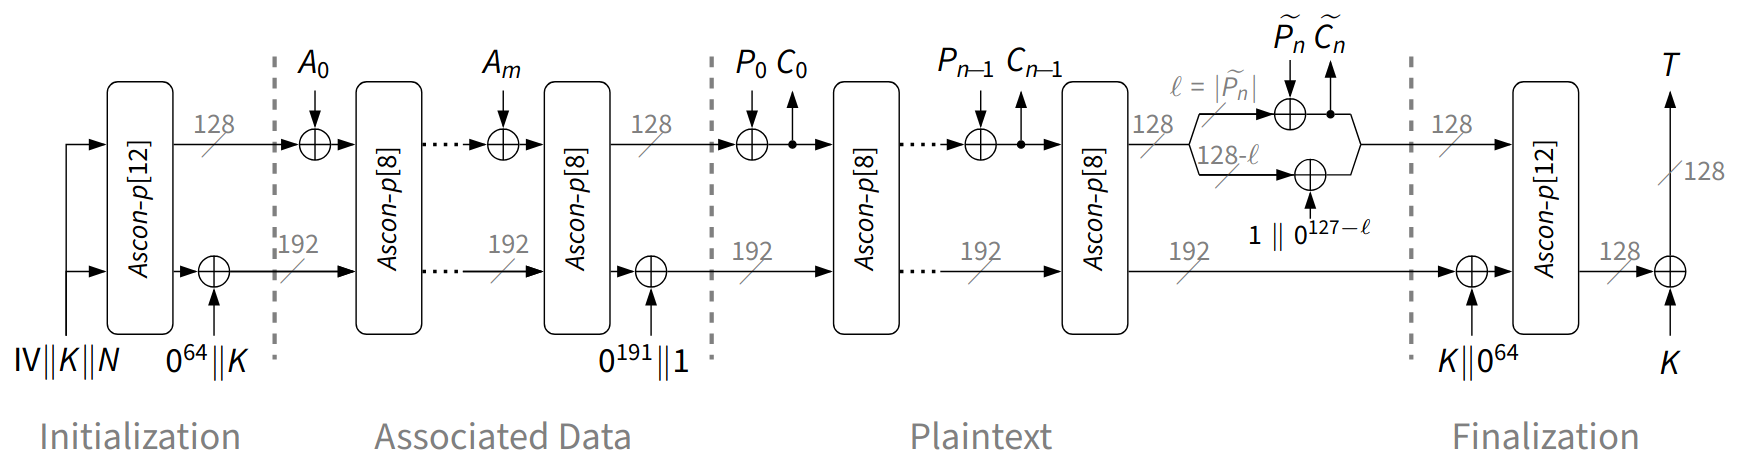
\includegraphics[scale=0.25]{felipe/figuras/fluxo-ascon-aead128-encript.png}
  \end{center}
  \legend{Fonte: \cite{nist2025ascon}}
\end{figure}

O processo de decifragem (Figura~\ref{fig:fluxo_ascon_decript}) possui uma estrutura muito semelhante à da cifragem. Ele passa pela mesma inicialização do estado de 320 bits e pelo processamento dos dados associados. A diferença principal ocorre nas etapas finais. O texto cifrado é processado bloco a bloco para recuperar o texto original e, na fase de finalização, a chave secreta é combinada com o estado interno para recalcular a \textit{tag} de autenticação. Se a \textit{tag} recalculada for idêntica à \textit{tag} recebida, o texto decifrado é considerado autêntico e é retornado, caso contrário, a mensagem é descartada.

\begin{figure}[htb]
  \caption{\label{fig:fluxo_ascon_decript}Processo de decifragem do Ascon-AEAD128}
  \begin{center}
    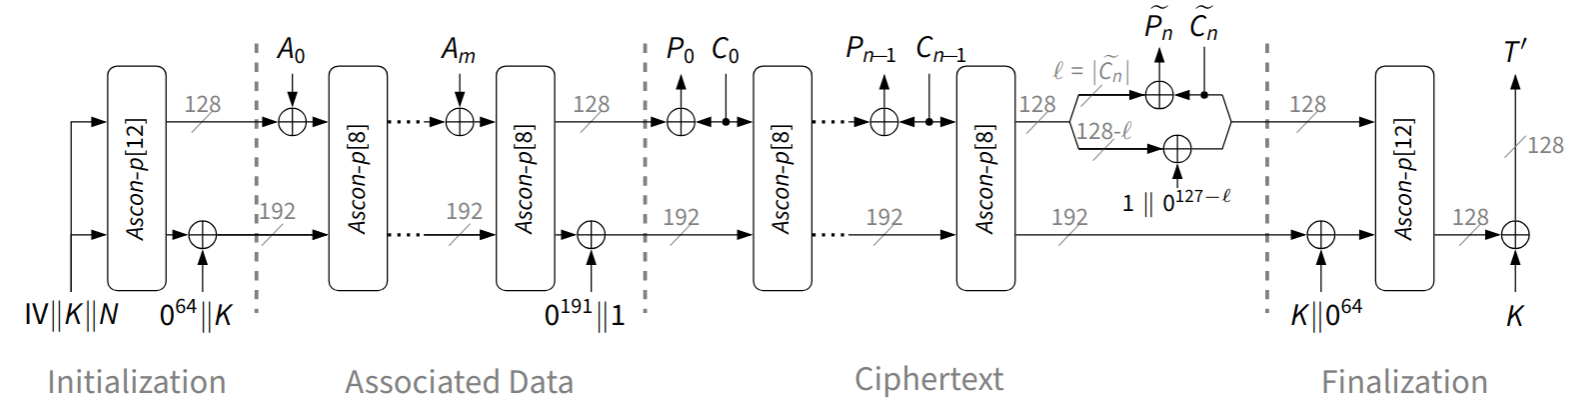
\includegraphics[scale=0.35]{felipe/figuras/fluxo-ascon-aead128-decript.png}
  \end{center}
  \legend{Fonte: \cite{nist2025ascon}}
\end{figure}

%%%%%%%%%%%%%%%%%%%%%%%%%%%%%%%%%%%%%%%%%%%%%%%%%%%%

\subsection{Comparativo de Algoritmos Criptográficos para IoT}
Durante a pesquisa inicial sobre criptografia leve, outros algoritmos foram avaliados, mas nenhum se mostrou tão adequado às necessidades do projeto quanto o padrão Ascon. Entre as principais alternativas analisadas, destacam-se o Speck \cite{beaulieu2013speck} e o ChaCha20 \cite{bernstein2008chacha}.

O Speck é uma cifra de bloco pura e bastante leve. No entanto, ele possui uma limitação estrutural importante para redes modernas, pois não oferece Criptografia Autenticada com Dados Associados (\textit{AEAD}) de forma nativa. Para garantir a integridade da mensagem, seria necessária a adição de um algoritmo de autenticação secundário e independente (como um código de autenticação de mensagem, MAC). O Speck teve sua padronização internacional ativamente rejeitada pela ISO (\textit{International Organization for Standardization}) por falta de transparência em seu design \cite{register2018nsa}.

O ChaCha20, por sua vez, é uma cifra de fluxo de altíssimo desempenho, amplamente adotada como padrão da indústria para cenários de \textit{software} onde \textbf{não} há aceleração de \textit{hardware} disponível. Contudo, assim como o Speck, ele carece de propriedades \textit{AEAD} embutidas. A exigência extra de se acoplar o algoritmo Poly1305 consome memória e processamento. Assim, ele não atende ao requisito de reunir confidencialidade, integridade e autenticidade em uma única operação, oferecido nativamente pelo Ascon.

Para a análise comparativa de viabilidade, este trabalho também optou por não focar nos demais algoritmos finalistas do processo de padronização do NIST (como TinyJAMBU ou Xoodyak) \cite{nist_lwc_finalists}, uma vez que o próprio comitê apontou o Ascon como o mais maduro dos finalistas em termos de segurança e como a submissão com maior volume de análise independente, no relatório oficial NIST IR 8454 \cite{nistir8454}.

Dessa forma, a metodologia de comparação deste trabalho foi refinada para responder à questão prática sobre o embate entre o novo padrão de \textit{software} e o padrão legado de \textit{hardware}. Os testes comparam exclusivamente o Ascon (novo padrão \textit{Lightweight Cryptography} do NIST) contra o AES-128-GCM (\textit{Galois/Counter Mode}), cujo bloco de cifra é executado no coprocessador de \textit{hardware} do microcontrolador, enquanto a autenticação (GHASH) permanece em \textit{software}. Essa abordagem permite avaliar se a migração para a criptografia leve em \textit{software} traz vantagens reais de consumo, memória e latência frente ao uso do acelerador de silício já embutido nas placas comerciais utilizadas em redes \textit{LoRaWAN}.

%%%%%%%%%%%%%%%%%%%%%%%%%%%%%%%%%%%%%%%%%%%%%%%%%%%%
%%%%%%%%%%%%%%%%%%%%%%%%%%%%%%%%%%%%%%%%%%%%%%%%%%%%
